\documentclass[10pt]{beamer}
\usepackage[utf8]{inputenc}
\usepackage{hyperref}

\usepackage{graphicx}
\usepackage[absolute,overlay]{textpos}

\mode<presentation> {
\usetheme{boxes} % When headline is wanted use Dresden theme instead
\usecolortheme{seagull}
%\logo{
\includegraphics[height=1.5cm]{ku_logo_dk}}
% \setbeamertemplate{footline}[frame number]
\setbeamertemplate{footline}{
  \hspace{1em}
  \hfill
  \insertframenumber/\inserttotalframenumber
  \vspace{1em}
  \hspace{1em}
  
\includegraphics[height=2cm]{ku_logo_dk}
  \hspace{1em}
}
\setbeamertemplate{navigation symbols}{}
\setbeamertemplate{itemize items}[square]
}






%----------------------------------------------------------------------------------------
%	TITLE PAGE
%----------------------------------------------------------------------------------------

\title[Kickstart-kursus] % bottom of every slide
  {Kickstart-kursus i programmering 2022} % title page

\author{\footnotesize{Daniel Spikol \& Martin Dybdal} \\
          \footnotesize{\texttt{ds@di.ku.dk}}}

\institute {
DIKU \\ Københavns Universitet
}

\date[9. august 2022]{9. august 2022}

\begin{document}
\begin{frame}[plain]
\titlepage
\end{frame}

% Hej venner. Velkommen på datalogi. Mit navn er Martin Dybdal og jeg
% skal guide jer igennem de næste 2 uger. Jeg er glad for at I valgte
% at komme til det her valgfrie kursus, og håber I kommer til at lære
% en masse. Både om at programmere og om hvordan man nemmest lærer at
% programmere.

% INTRO AF INSTRUKTORER

% Formålet med kurset er at I ikke føler jeg helt så meget på dybt
% vand, når semesteret for alvor starter. Det betyder ikke at vi lærer
% jer det samme som når de rigtige kurser går i gang, men forhåbentlig
% kan mange af de ting i lærer i denne uge alligevel gøre det nemmere
% at bevare overblikket når det pludselig går rigtig stærkt og der er
% ugentlige afleveringsopgaver.

% De her to uger skal vi bare hygge os, der kommer ikke til at være
% afleveringer, pensum eller prøver. Vi vurderer i fællesskab om det
% vi laver virker ved at afprøve og lege med det. Jeg tænker vi skal
% bare rigtig hurtigt i gang, så vi får mest ud af tiden, i stedet for
% at jeg plabrer så meget mere. Vi tager nogle pauser i løbet af
% dagen, og vi går en fælles tur over til Jura-kantinen kl. 12

%%% SLIDES om DAGSplan og Socialt

% De første dage skal lege med computergrafik, computerkunst og
% computerspil. Senere putter vi også noget elektronik på. Vi skal
% bruge programmeringssproget Python. Inden jeg fortæller mere om
% kurset, vil jeg gerne have jer alle sammen på internettet og så have
% jer til at udfylde det spørgeskema jeg har lagt op inde på Absalon.


\section{Intro til kurset}
% \begin{frame}
%   \frametitle{Velkommen!}

%   \begin{itemize}
%   \item Præsentation af undervisere
%   \item Hvorfor et kickstart-kursus?

%     % De andre fag er heldige at have fag i skolen og gymnasiet, og
%     % kan forvente at de studerende allerede kan
%     % Det kan vi ikke, så vi kan ikke hold et brush-up kursus, som de
%     % andre, hvor vi bare skal genopfriske, så vi starter fra bunden
%   \end{itemize}

% \end{frame}


\begin{frame}
  \frametitle{Daglig plan}
  \begin{itemize}
  \item kl. 9:00-12:00 - Mini-lektion, kode, kode, kode
  \item kl. 12:00 - frokost
  \item kl. 13:00-14:40 - kode, kode, kode
  \item kl. 14:40-15:00 - opsamling på dagen
  \item kl. 15:00-? - Arbejd eventuelt videre, hjælp hinanden, slap af til næste dag
  \end{itemize}

\end{frame}


\section{Internetadgang og Installation}
\begin{frame}
  \frametitle{Internetadgang}

  Aktiver KU-bruger
  \begin{itemize}
  \item Log på \texttt{http://mit.ku.dk} med NemID og find midlertidig pinkode.
  \item Gå til \texttt{http://kunet.dk} og tryk ``Første gang du logger på''.
  \item Log på med den midlertidige kode og CPR nummer uden bindestreg.
  \item Aflæs KU brugernavn (fx \texttt{abc123}) og angiv password.
  \end{itemize}

  \vspace{5mm} 
  eduroam WiFi
  \begin{itemize}
  \item Kræver KU bruger og password
  \item Log på med brugernavn: \texttt{abc123@ku.dk}
  \end{itemize}

  \vspace{5mm} 
  Alternativt: KU Guest WiFi
  \begin{itemize}
  \item Opret 24 timers konto ved at indtaste navn, mail, mobilnummer. 
  \item Modtag kode via SMS.
  \end{itemize}
  %   \begin{textblock}{5}(2,2)
% \end{textblock}
\end{frame}

\begin{frame}
  \frametitle{Spørgeskema}
  \begin{itemize}
  \item Log på \url{http://absalon.ku.dk}
  \item Gå ind på kursussiden
  \item Klik på ``Tests'' / ``Quizzes''
  \item Brug de næste 15 min på at udfylde spørgeskemaundersøgelsen
  \end{itemize}

\end{frame}

\begin{frame}
  \frametitle{Socialt}
  \begin{itemize}
  \item Lær hinanden at kende
  \item Spørg hinanden før i spørger en underviser.
  \item Hjælp andre hvis I er hurtige. Man lærer også ved at sætte ord
    på og forklare videre.
  \item Skriv et navneskilt.
  \end{itemize}

  \vspace{1cm}
  Arrangementer
  \begin{itemize}
  \item Torsdag kl. 17: Studenterrådet afholder rusarrangement for
    alle nye studerende (her i bygningen). Mød rusvejledere, mentorer m.m.
  \item Fredag: hygge ved vandet ved Islands Brygge?
  \end{itemize}
\end{frame}

\begin{frame}
  \frametitle{Tema for kurset}
     Hvordan kan vi få borgerne til at ændre
     adfærd i forhold til at bruge grøn energi?
  
  %TODO : Fotos/screenshots af projekter.

\end{frame}

\begin{frame}
  \frametitle{Installation af Processing.py}

  \begin{itemize}
  \item Hent og installer Processing fra \url{http://processing.org/download/}
  \item Installer Python Mode via
  \end{itemize}
  %   \begin{textblock}{5}(2,2)
% \end{textblock}
\end{frame}

\section{Processing}
\begin{frame}
  \frametitle{Processings koordinatsystem}

  \vspace{3mm}
  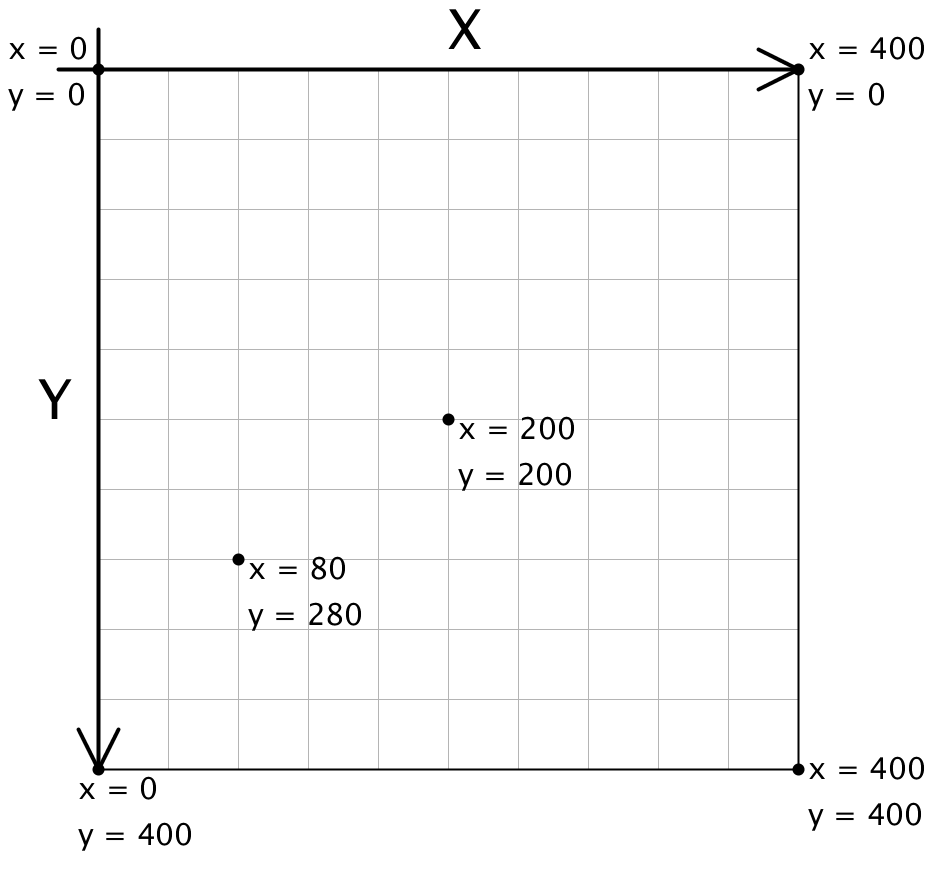
\includegraphics[width=0.8\textwidth]{../arbejdsark/illustrationer/koordinatsystem}

\end{frame}

\begin{frame}
   \frametitle{Today's Recap}
   	\begin{itemize}
	\item Marshmallow Challenge
	\begin{itemize}
	\item constant prototyping as a problem-solving method
	\item \href{https://www.ted.com/talks/tom_wujec_build_a_tower_build_a_team?utm_campaign=tedspread&utm_medium=referral&utm_source=tedcomshare}{TED TALK Tom Wujec}
	\end{itemize}
	\item Coordinate System 
	\item Drawing with Processing
	\item Variables
	\item Functions
	\end{itemize}
\end{frame}

 \begin{frame}
   \frametitle{Thinking about tomorrow}
   \begin{itemize}
   \item \href{https://en.wikipedia.org/wiki/Pair_programming}{Wikipedia: Pair Programming}
   \item \href{https://youtu.be/ET3Q6zNK3Io}{Video}
   \item \href{https://medium.com/@volkanbier_42259/how-to-put-pair-programming-into-action-ce9ebb9d711
   \end{itemize}
   \end{frame}



\end{document}